\graphicspath{{images/tn-gp-sagit/drafts/}}

\chapter{Study IV: Gaussian Process Classification of Trigeminal Neuralgia With Merged Tractography}
\chaptermark{Study IV}

\section{Abstract}
\textbf{Introduction:} Trigeminal Neuralgia (TN) is a debilitating facial neuropathic pain syndrome involving the trigeminal sensory pathway. We demonstrate the use of a fully-automated group white-matter tractography, and Gaussian Process (GP) classification to pinpoint key white-matter diffusivity changes that maximally differentiate patients and healthy controls. 

\textbf{Methods:} We performed group merged tractography using SAGIT on 36 sex-matched TN patients (right-sided pain) and 36 controls. The trigeminal nerve (CN V), pontine decussation, and thalamocortical S1 pathways were reconstructed. GP classifiers were trained by scrolling a moving window over CN V and S1 tractography centroids. FA, GFA, RD, AD, and MD metrics were evaluated. Both TN vs. Control and Affect vs. Unaffected were analyzed. Classifiers that performed at greater-or-equal-to 75\% accuracy were accepted.

\textbf{Results:} Both affected and unaffected trigeminal nerves in TN patients can be differentiated with up to 80\% accuracy from controls. Affected CN V differences were more focused in the cistern and root-transition-zone, whereas unaffected CN V show more focus towards the brainstem. The affected S1 showed focused MD differences towards the cortex with an accuracy of 85\%. 

\textbf{Conclusions:} We have demonstrated the first instance of group-wise merged tractography analysis of TN vs. control,  as well as the first white-matter machine learning classification with GP. The method reproduced previous findings with finer-grained regional specificity. The study also revealed specific diffusivity changes in deeper white matter.

\section{Introduction}
\subsubsection{Trigeminal Neuralgia}
Trigeminal neuralgia (TN) is a debilitating facial neuropathic pain syndrome characterized by paroxysmal and shock-like pain in one or more dermatomes of the three trigeminal nerve (The fifth cranial nerve: CN V) branches. TN manifests classically in idiopathic fashion, or secondary to a range of neuropathology, including meningiomas \cite{Cheng2008}, trigeminal schwannomas \cite{Miller2008}, neurocysticercosis \cite{Revuelta1995}, and most notably multiple-sclerosis (MS) \cite{Cruccu2009,VanderMeijs2002,Nick2012}. The pathophysiology of idiopathic TN is thought to be vascular compression at the root of the CN V nerve entry zone (NEZ) \cite{Linn2011,Love2001}, although idiopathic TN can also occur without evidence of vascular compression \cite{Lee2014}. We previously compared TN and MS-TN diffusivity differences in four segments of the CN V at the level of the pons \cite{Chen2016a}, and confirmed that brainstem CN V diffusivity is disrupted in MS-TN. In all previous TN studies, placements of region-of-interests in the CN V were pre-determined and manually placed. In this study we further expand the study to A) analyze the CN V differences between TN and healthy controls across the entire nerve using along-the-track and machine-learning methods to auto-discover key regions-of-interest; B) extend the examined regions to include trigeminopontothalamic (TPT) and thalamocortical (S1) white matter pathways as part of the trigeminal sensory pathways.

The trigeminal sensory system involves both the discriminative touch and pain pathways. The discriminative pathway synapsis onto the primary trigeminal sensory nucleus, and then project to the contralateral VC thalamus, and then to the S1 cortex as we have delineated. The pain pathway synapsis caudally onto the trigeminal spinal nucleus, and decussate at the level of the medulla and spinal cord. The pathway merges with the discriminative sensory pathway and ascend as the contralateral trigeminal lemniscus, and also project to the contralateral VC thalamus. The pain pathway also projects to the medial nucleus of the thalamus, where it then project medially to the cingulate cortex. 

\subsubsection{Data Analysis from Streamlines}
Neuroimaging tractography is commonly used for anatomical visualization \cite{Chen2011b}, white matter segmentation \cite{Behrens2003a,Johansen-Berg2005}, and structural connectivity analysis \cite{Cao2013,Wiech2014}. To obtain diffusivity metrics from tractography involves converting the streamline bundles into a volumetric spatial mask, and then measure the mean metric from all or parts of the masked voxels \cite{Concha2005,Fitzsimmons2009}. However this approach discards the orientation information in the streamlines. The naive form of spatial masking is to identify voxels where at least one streamline has passed through it, which often results in identifying voxels with minimal streamline pass-through. This becomes an issue when considering that an average 3-tesla HARDI DWI acquisition has a voxel dimension of 2 to 3 mm. In white matter structures such as CN V, and other small pathways, the structure diameter may be no more than 3mm, and therefore the naive spatial masking approach would result in severe partial volumes that will confound the result. 

Consider that a tractography streamline propagation algorithm involves all or parts of the following stages: 1) subsampling of an initial region for seeding \cite{Basser2002,Cote2012}; 2) identifying a propagation direction, based on previously traversed paths \cite{Malcolm2010,Qazi2009,Tournier2010}; 3) smoothing of the traversed paths for output \cite{Tuch2000d}. It is reasonable to consider these algorithms to be an interpolated subsampling scheme of the DWI volume that takes the diffusion-based orientation into account. Therefore, it is desirable to directly make use of the tractography streamlines for data measurement. 

Along-the-tract analysis has been investigated by various authors \cite{Colby2012,ODonnell2009,Wang2015,Yeatman2012}. In these approaches, the bundles are selectively filtered from global tractography \cite{Wang2015,Yeatman2012}, and studies were limited to major white matter bundles such as the corpus callosum, corticospinal tract, longitudinal fasciculus, arcuate fasciculus, and uncinate. The measures were pooled onto tract centroid in each individual subjects, and then aggregated at the group level. The global tractography approach is unintuitive for anatomy-specific tasks such as neurosurgical planning, where the anatomy of interest is clear. A more focused ROI based delineation approach is therefore preferred in these circumstances.

It is important to note that streamline clustering and centroid identification can be considered as independent tasks. Some clustering methods do not provide a best-representative streamline centroid. Centroid identification involved resampling the streamlines into an identical number of points, and then identifying point correspondences via different distance measures. For these approaches, it is vital that the streamlines have similar length, and an assumption that the start and end of the streamlines across subjects are consistent. However, pathological brain tissue may negatively affect tractography delineation. Therefore the geometry assumptions of such approaches may not be satisfied when extending them to study patient populations. Running time and memory constraints also need to be taken into consideration, when applying such algorithms at a group level. One method for tract clustering and centroid identification that is shown to have linear running time in respect to streamline count is QuickBundles \cite{Garyfallidis2012}. We have adopted QuickBundles to obtain S1 streamline centroids. 

The principal advantage of a streamline-based approach is that we can retain the pathway orientation from its geometry. White matter metrics in 3D space can then be projected to a lower dimensional centroid for detailed analysis. We have developed the Selective Automated Group Integrated Tractography (SAGIT) framework (Chen et al., 2016) to automate group-wise tractography delineation, which ensures consistent region-of-interest projection, tractography seeding sampling scheme, and tractography parameter tuning. We then merge the tracts into a template space using non-linear deformations, and then perform tractography centroid identification and statistics at the merged group level to ensure anatomical consistency. 

\subsubsection{Gaussian Process}
The breakthrough results of deep convolutional neural networks in computer vision \cite{Krizhevsky2012} have sparked the interest of deploying similar systems for medical imaging diagnosis \cite{Greenspan2016}. However, one disadvantage of DNN is in its inability to quantify uncertainty and provide interpretable models. Model interpretability is a fundamental requirement for machine learning in medicine, and therefore there is renewed interest in bayesian-based models like Gaussian Process (GP) \cite{gal2016dropout}. In fact, it has been found that DNN with an infinite number of hidden units approximates GP \cite{neal1996priors}. 

Gaussian Process is defined \cite{rasmussen2006gaussian}) as a collection of random variables, any finite number of which have a joint Gaussian distribution. 
It is a distribution that is defined by a mean function $m(x)$ and covariance function $k(x,x') $ where
\begin{equation}
	\begin{split}
		m(x) &= \mathbb{E}[f(x)], \\
		k(x,x') &= \mathbb{E}[(f(x)-m(x)(f(x')-m(x'))],
	\end{split}
\end{equation}
And the Gaussain processed is defined as
\begin{equation}
f(x) \sim GP(m(x), k(x, x')) 
\end{equation}

The covariance function is also termed called kernel function. The radial-basis function kernel or RBF kernel is widely used in machine learning tasks. GP has previously been explored in neuroimaging for tractography clustering \cite{Wassermann2010}. It is particularly well suited for continuous data streams, such as tractography streamlines. 

\section{Methods}
\subsubsection{Acquisitions}
The study recruited 36 idiopathic TN patients (28 females, 8 males; age 60.1$\pm$16 years; all right side pain), and 36 healthy controls (28 females, 8 males, age 42.7$\pm$12 years).  All TN patients were scanned at 1 day pre-GK and 6 months post-GK. MRI acquisitions including T1 fast-spoiled gradient echo (FSPGR) and diffusion weighted image (DWI) acquisitions. T1 scans were acquired with 1mm slice thickness, in-plane resolution of 0.9375x0.9375mm, slice spacing=1 mm, TE=5.052 ms, TR=11.956 ms, flip angle=20 deg, FOV=240 mm, and matrix=256x256. DWI scans were acquired with 1 B0 scan, 60 gradient directions, 3mm slice thickness and an in-plane resolution of 0.9375x0.9375 mm, b0=1000 s/mm2, TE=88.6 ms, TR=17000 ms, flip angle=90 deg, field of view (FOV)=120 mm, and matrix=128x128.

\subsubsection{Preprocessing}
DWI images were motion/eddy-current corrected, with appropriate correction applied to the b-matrix \cite{Leemans2009}. Region of interests (ROI) for tractography seeding were manually created on a normalized template brain from 42 healthy brains. The normalized brain template was created using Anatomical Normalization Tools \cite{Avants2010,Avants2011}. 

We deployed selective automatic group integrated tractography (SAGIT) framework to automate preprocessing, registration, and tractography. The processing steps are as follows: T1 anatomical images were processed using FreeSurfer \cite{Fischl2004} for cortical and subcortical segmentations. The T1 images for all the subjects were registered to the template using symmetric diffeomorphic registration (SDR) \cite{Avants2008b}. Each individual DWI was registered to their T1 image with SDR, using mean DWI image for DWI-T1 co-registration. Freesurfer segmentation maps were first affine transformed from the Freesurfer space to the T1 space using FMRIB's Linear Image Registration Tool (FLIRT) \cite{Jenkinson2001,Jenkinson2002}, and then transformed using SDR transforms to the individual DWI space for selective ROI generation with SAGIT.

\subsubsection{Tractography}
ROIs were defined on the template image to bilaterally delineate: 1) CN V (ROI: cistern nerve root; excludes: cerebellum grey matter, pontine cerebellar peduncles); 2) trigeminothalamic pontine decussation (TPT) (ROIs: trigeminal nucleus (TGN); includes: contralateral VC thalamus, pontine decussation; excludes: ipsilateral thalamus, cerebellar grey matter, pons, contra-lateral S1 ); 3) thalamocortical S1 pathway (ROIs: VC thalamus; includes: ipsilateral S1 white-matter boundary; excludes: brainstem).  

Constrained spherical deconvolutional tractography (CST) \cite{Tournier2012b} was used to delineate the three sets of anatomy. Deterministic CST was applied to delineate CN V and S1 anatomy, while probabilistic (iFOD2) CST \cite{Jeurissen2011b,Tournier2010} was applied to delineate TPT anatomy. Deterministic CST was performed with step size = 0.3mm, angle threshold = 45$\deg$, streamline count=200, minimal length = 5 mm, initial cut-off = 0.1, cut-off = 0.1, and with 4th-order Runge-Kutta integration. Probabilistic tractography for S1 projection was performed with step size = 5mm, angle threshold = 45$\deg$, streamline count = 300, max number of stream generation = 1 million, minimal length = 10 mm, maximum lengh = 80 mm, initial cut-off = 0.15, cut-off = 0.15. Probabilistic tractography for TPT project was performed with step size = 1mm, and streamline count = 2000, and maximal length = 60 mm. 

Tractography was first performed in the native DWI space for each individual.  FA, AD, RD, MD, and GFA metrics were embedded into the native tractography models by sampling the corresponding images maps using the points of the tractography geometry with tri-linear interpolation. Additionally, subject ID and group ID scalar values were also inserted into each tractography files for identification. 

\subsubsection{Merged Tractography}
All tractography delineations of the same anatomy across all the subjects and groups were merged into a single tractography file for analysis. A software library called “Fascicles” is created by the author to facilitate this process. The individual tract files were converted into a SQLite relational database \cite{owens2010sqlite}, and then all points were exported into a comma-delimited file. The points were then transformed by applying the subject DWI to T1, and T1 to template transforms using ANTs’  applyTransformToPoints command \cite{Avants2009}. The transformed points were then imported back into the SQLite database, and a new template-space tractography model is exported using the transformed point-set, with all its original scalars and subject/group ID associations preserved. Finally, all template-space tractography models across all the subjects are imported into a new SQLite database, and then exported as a single file for analysis. 

\subsubsection{Along-the-tract Analysis}
The merged tract was first post-processed in 3D Slicer to remove erroneous and stray streamlines that will confound measurement. Streamlines removed include remnant CN V streamlines that stray into the cerebellar peduncles or other non-TGN regions, and streamlines that are perpendicular to the nerve in the cisternal space that appear to be partial delineation of vessels or noise. S1 streamlines that stray medially towards other regions such as the corpus callosum were also removed. The TPT streamlines were not examined due to inconsistent reproducibility across subjects. 

Tractography centroids, which were the average curve best fit the tract bundle, was defined on the merged tracts in template space. CN V centroids were manually defined. The CN V centroids were defined by a list of 3 control points situated in the template world space. A Catmull-Rom spline \cite{DeRose1988} was then defined from these control points using the VTK software library \cite{Schroeder2005}, which resulted in a curve of length 38.91 mm. The spline is then resampled into 30 points that become the centroid definition with segment length of 1.3 mm. Nearest-neighbor point assignment was used to divide the merged tract into 30 cross sections along the centroids. Diffusion metrics from the points were aggregated for each of the cross-sections.  S1 centroids were defined using QuickBundles \cite{Garyfallidis2012} with distance threshold of 30, with centroid length of 62.1 mm and segment length of 2.07 mm. 

\subsubsection{Gaussian Process Classification}

Diffusivity metrics of affected (right side) and unaffected CN V and S1 pathways were independently compared with those of controls, where control metrics were the average of both left and right sides. The affected and unaffected sides in TN patients were also compared with each other. 
Age was regressed out by using the residuals of the linear regression model from the controls group. The diffusion values were subsequently normalized to zero mean with ranges $[-1, 1]$ for model training. 
Gaussian Process (GP) classification was exhaustively performed on CN V and S1 nerve segments to identify key segment differences. Multiple moving windows of length between 5 to 30 were used to constraint tract segments, and a Gaussian Process model was trained for each windowed segment. The entire machine learning process was performed using Scikit-learn machine learning software framework.
For each model, the subjects were split into train and validation sets using stratified 10-fold cross-validation. The GP model was initiated with Matern kernel (length scale = 1), and the model fitted using the training set. The validation set was used to measure prediction accuracy, and the mean accuracy of the 10-fold cross-validation was used to assess the windowed segment. Segments accuracy greater than 75\% were accepted, and the segment length with the greatest accuracy was then determined. 

\subsection{Results}
\subsubsection{Group Tractography}
Merged CN V delineations show anatomical consistency, and extended into the ipsilateral TGN. Changes in FA along the streamlines demonstrate clear differences between cistern and brainstem segments, suggesting good agreement in anatomical registration ( Figure \ref{fig:GPfigure1}). 
The TPT projections, when filtered strictly from the TGN to the ipsilateral VC thalamus region, showed distinct bundles of decussating pathways between left and right. The resulting pathway was not symmetrical, where the right TPT pathway diverts and envelopes the left (Figure \ref{fig:GPfigure2}). TPT streams lines were sparse, suggest low inter-subject reproducibility. Therefore no additional analysis was carried out for TPT.
S1 streamlines reliably extended into the face region of the S1 cortex (Figure \ref{fig:GPfigure3}). 

\begin{figure}[ht]
\centering
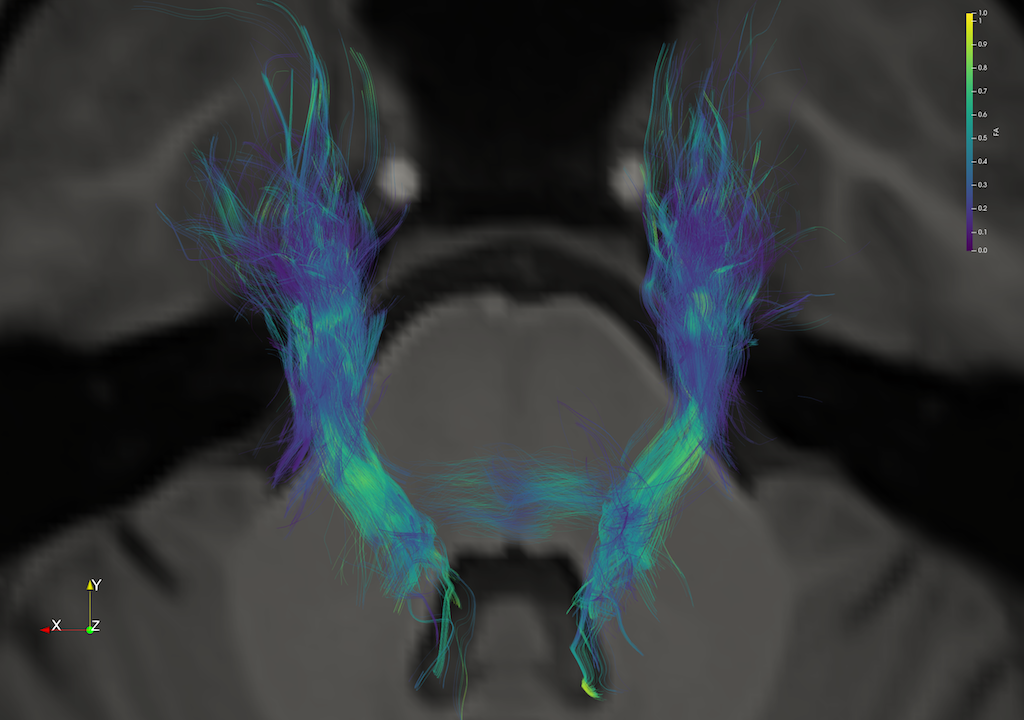
\includegraphics[width=\linewidth]{cnv-inferior-view.png}
\caption{Inferior view of the merged CN V delineations.}
\label{fig:GPfigure1}
\end{figure}

\begin{figure}[ht]
\centering
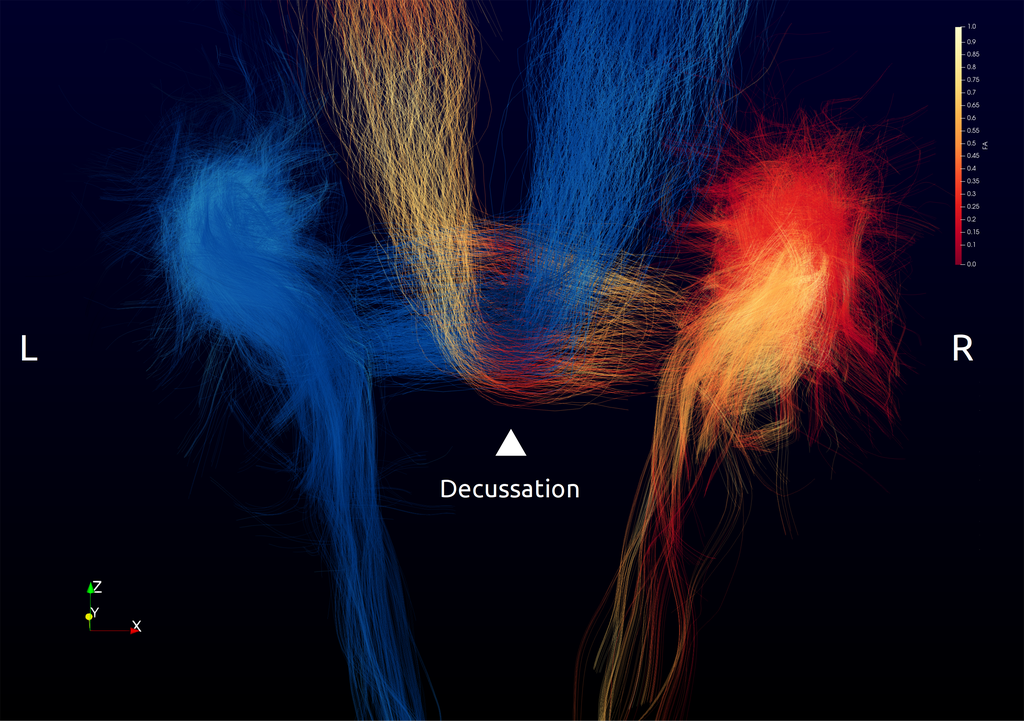
\includegraphics[width=\linewidth]{view-decussation.png}
\caption{Close up of the TPT decussation. Red: Right TPT; Blue: Left TPT. Note the Right TPT diverts around the left TPT bundle. }
\label{fig:GPfigure2}
\end{figure}

\begin{figure}[ht]
\centering
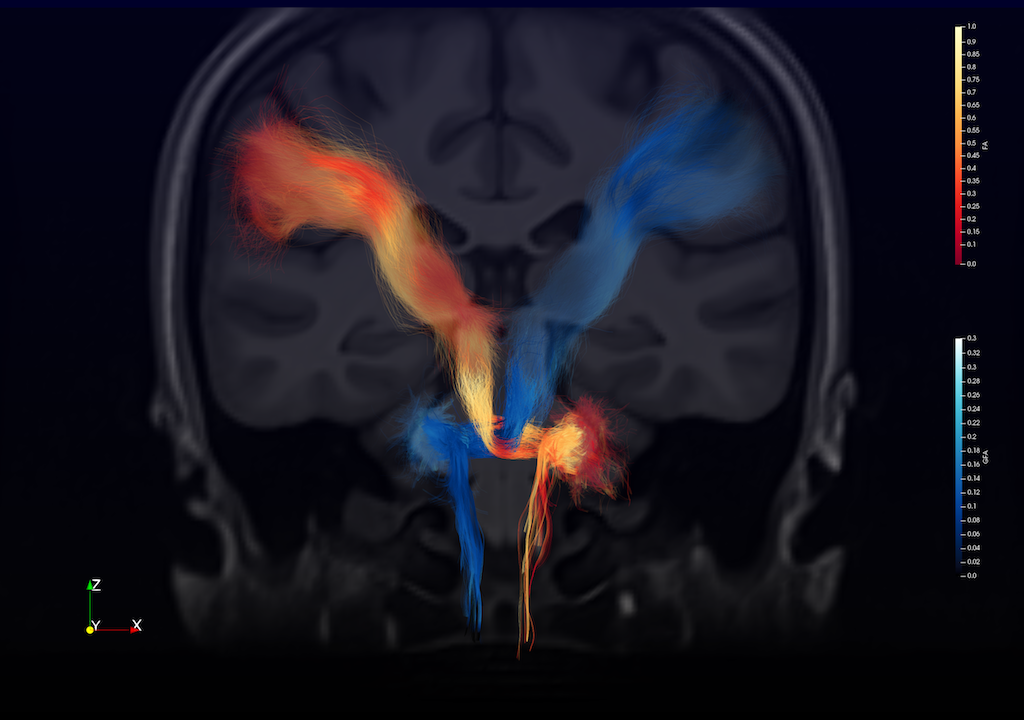
\includegraphics[width=\linewidth]{view-left-right.png}
\caption{The complete trigeminal discriminatory sensory pathway. }
\label{fig:GPfigure3}
\end{figure}

\subsubsection{CN V}
Both sides were distinguished from controls with classifiers that achieve greater than 75\% accuracy. 
Classifiers on the right side have performance ranging from 77\% (GFA) to 80\% (MD) accuracy. The left classifiers achieved accuracy ranging from 75\% (FA) to 80\%(GFA). The right side shows more consistent overlap of segment ranges between positions 10--17, in the region of the cistern/REZ; while the left side shows less consistent range overlaps, and AD segment range from positions 3 to 14, which include the brainstem regions. Overall, the right side features extend further into the distal space, into the cistern and even the ganglion, while the left side extends more into the brainstem. Comparing left/right, only the FA classifier achieved greater than 75\% accuracy, where its segments range from 11 to 19, which is the cisternal segment (Figure \ref{fig:GPfigure4}). 

The best performing segments versus controls is GFA (segment 8--14) on the left (unaffected) side, with 80\% accuracy, 84\% precision, and AUC of 0.8; while MD (segment 10--17) performed the best on the right (affected) side, with 80\% accuracy, 84\% precision, and AUC of 0.79 (Table \ref{table:CN V}, Figure \ref{fig:GPfigure6}). The best performing left-versus-right classifier was FA (segment 11--19), with 75\% accuracy, 82\% precision, and AUC of 0.75.

\begin{figure}[ht]
\centering
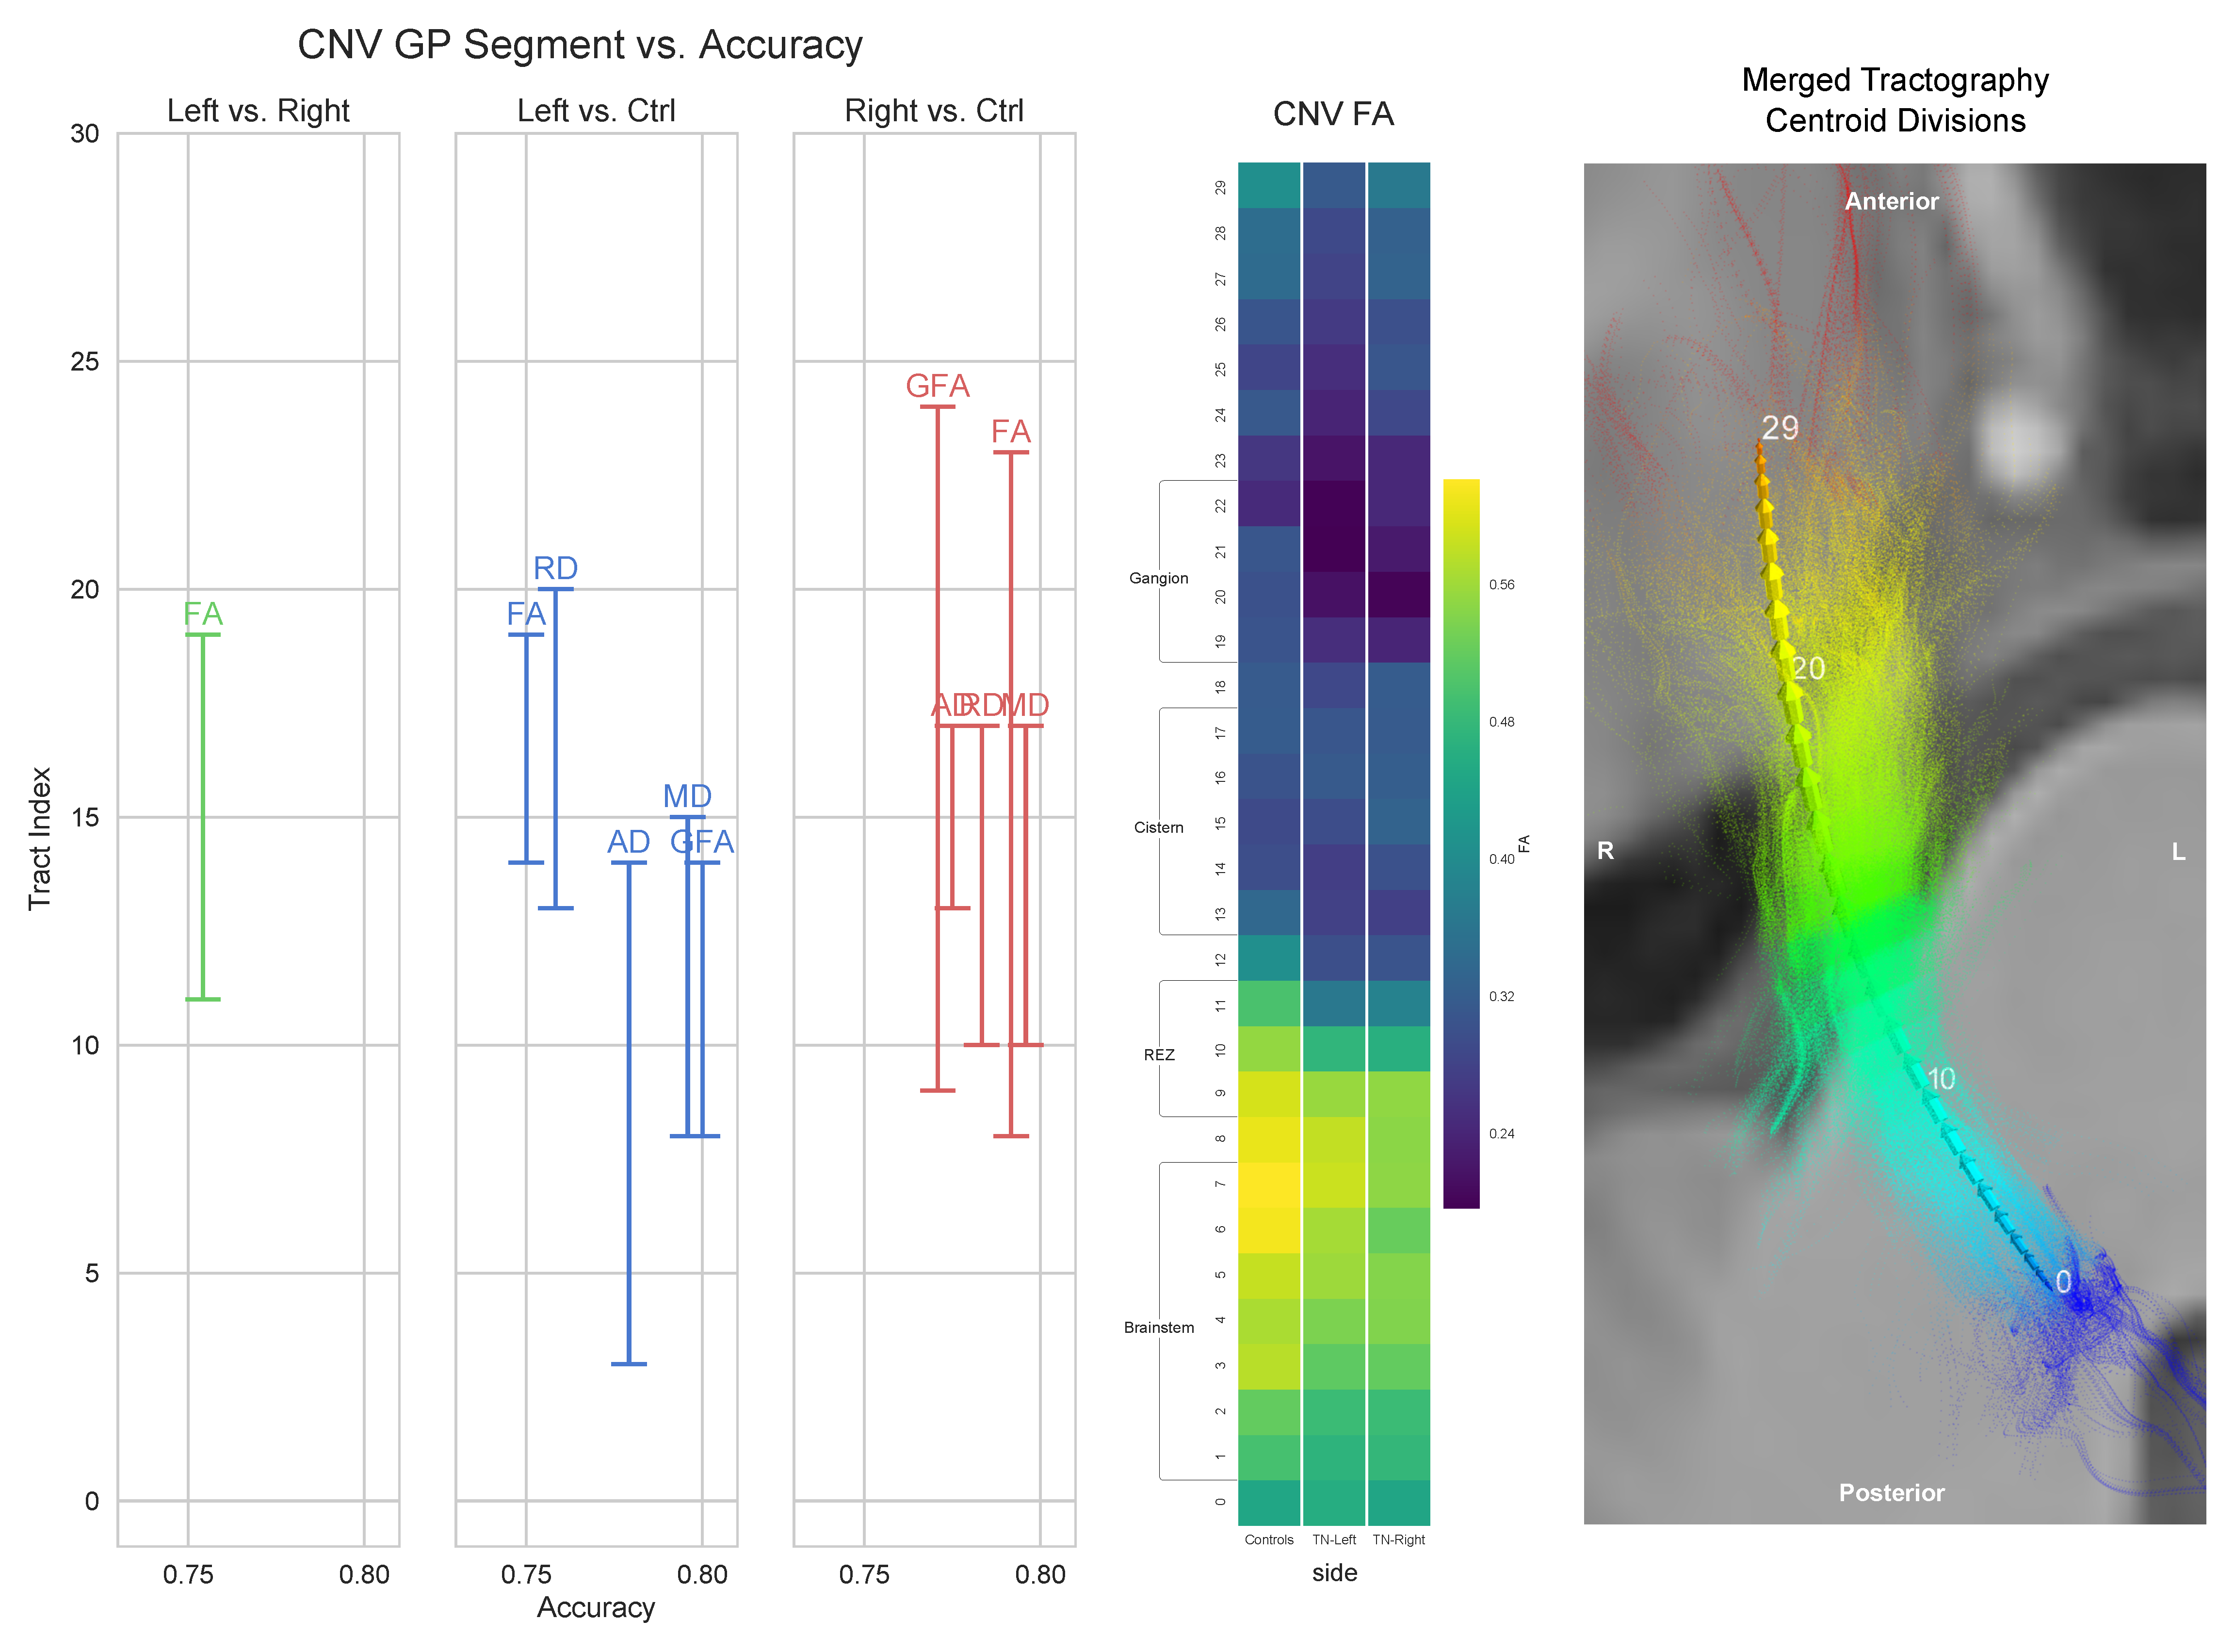
\includegraphics[width=\linewidth]{figure-GP-CNV.pdf}
\caption{CN V classifier performance}
\label{fig:GPfigure4}
\end{figure}

\begin{table}[ht]
\centering
\csvautotabular{cnv_table.csv}
\caption{CN V GP classifier performance data}
\caption*{List of the best accuracy for each diffusion metric. Precision, recall, and f1 scores are also provided for reference}
\label{table:CN V}
\end{table}

\subsubsection{S1}
Both sides of the S1 face region pathway were able to be distinguished by classifiers with greater than 75\% accuracy. 
The FA and RD classifiers at locations 617, representing the segment that emerge from the thalamus and merging into corona radiata, are common to both sides. The left side has higher classification accuracy of 80\% with FA, while the right side had a maximum accuracy of about 78\% with RD. 
The MD classifier meanwhile  is unique to the left side, and achieved an accuracy of 85\% in locations 16--23, near the grey-white matter boundary, closer to the cortex (Figure \ref{fig:GPfigure5}).

The best performing segment versus controls was MD (segment 16--23) on the left (affected) side, with 85\% accuracy, 88\% precision, and AUC of 0.83; whereas the best on the right (unaffected) side was FA (segment 6--16), with 78\% accuracy, 81\% precision, and AUC of 0.76 (Table \ref{table:s1}, Figure \ref{fig:GPfigure6}). 

\begin{figure}[ht]
\centering
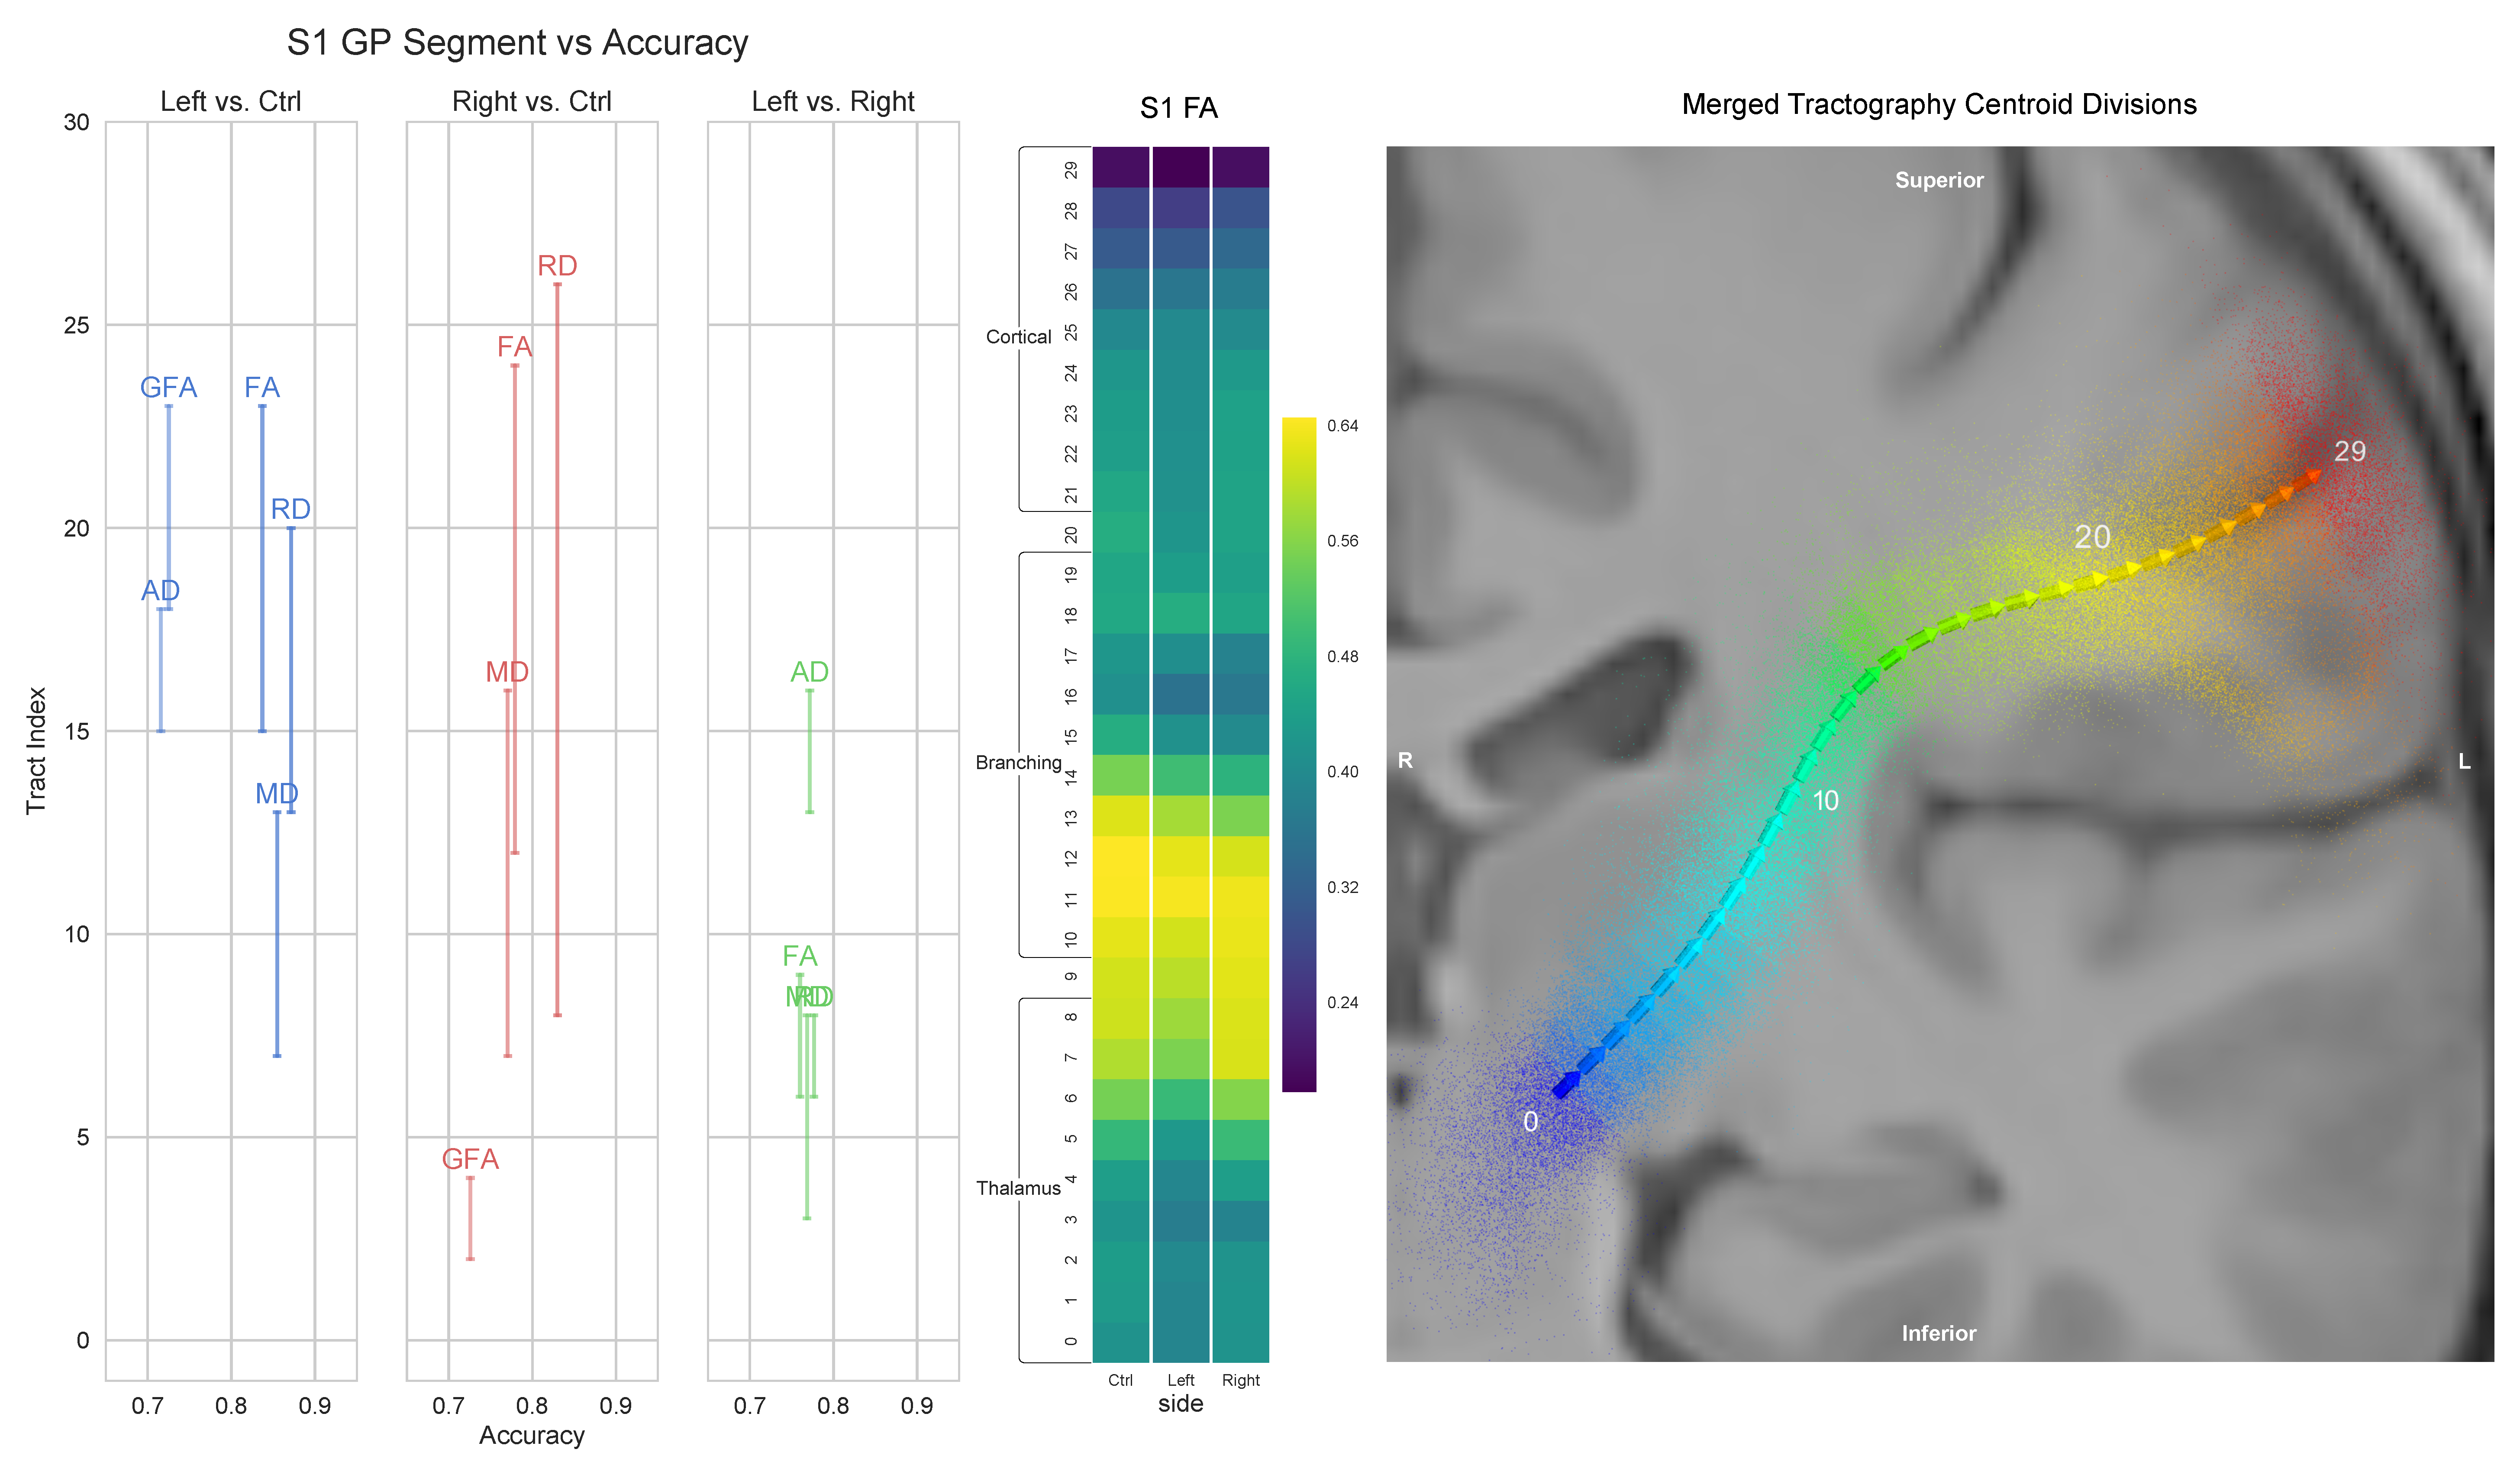
\includegraphics[width=\linewidth]{figure-GP-S1.pdf}
\caption{S1 classifier performance}
\label{fig:GPfigure5}
\end{figure}

\begin{table}[ht]
\centering
\csvautotabular{s1_table.csv}
\caption{S1 GP classifiers performance data}
\caption*{List of the best accuracies for each diffusion metric. Precision, recall, and f1 scores are also provided for reference}
\label{table:s1}
\end{table}

\begin{figure}[ht]
\centering
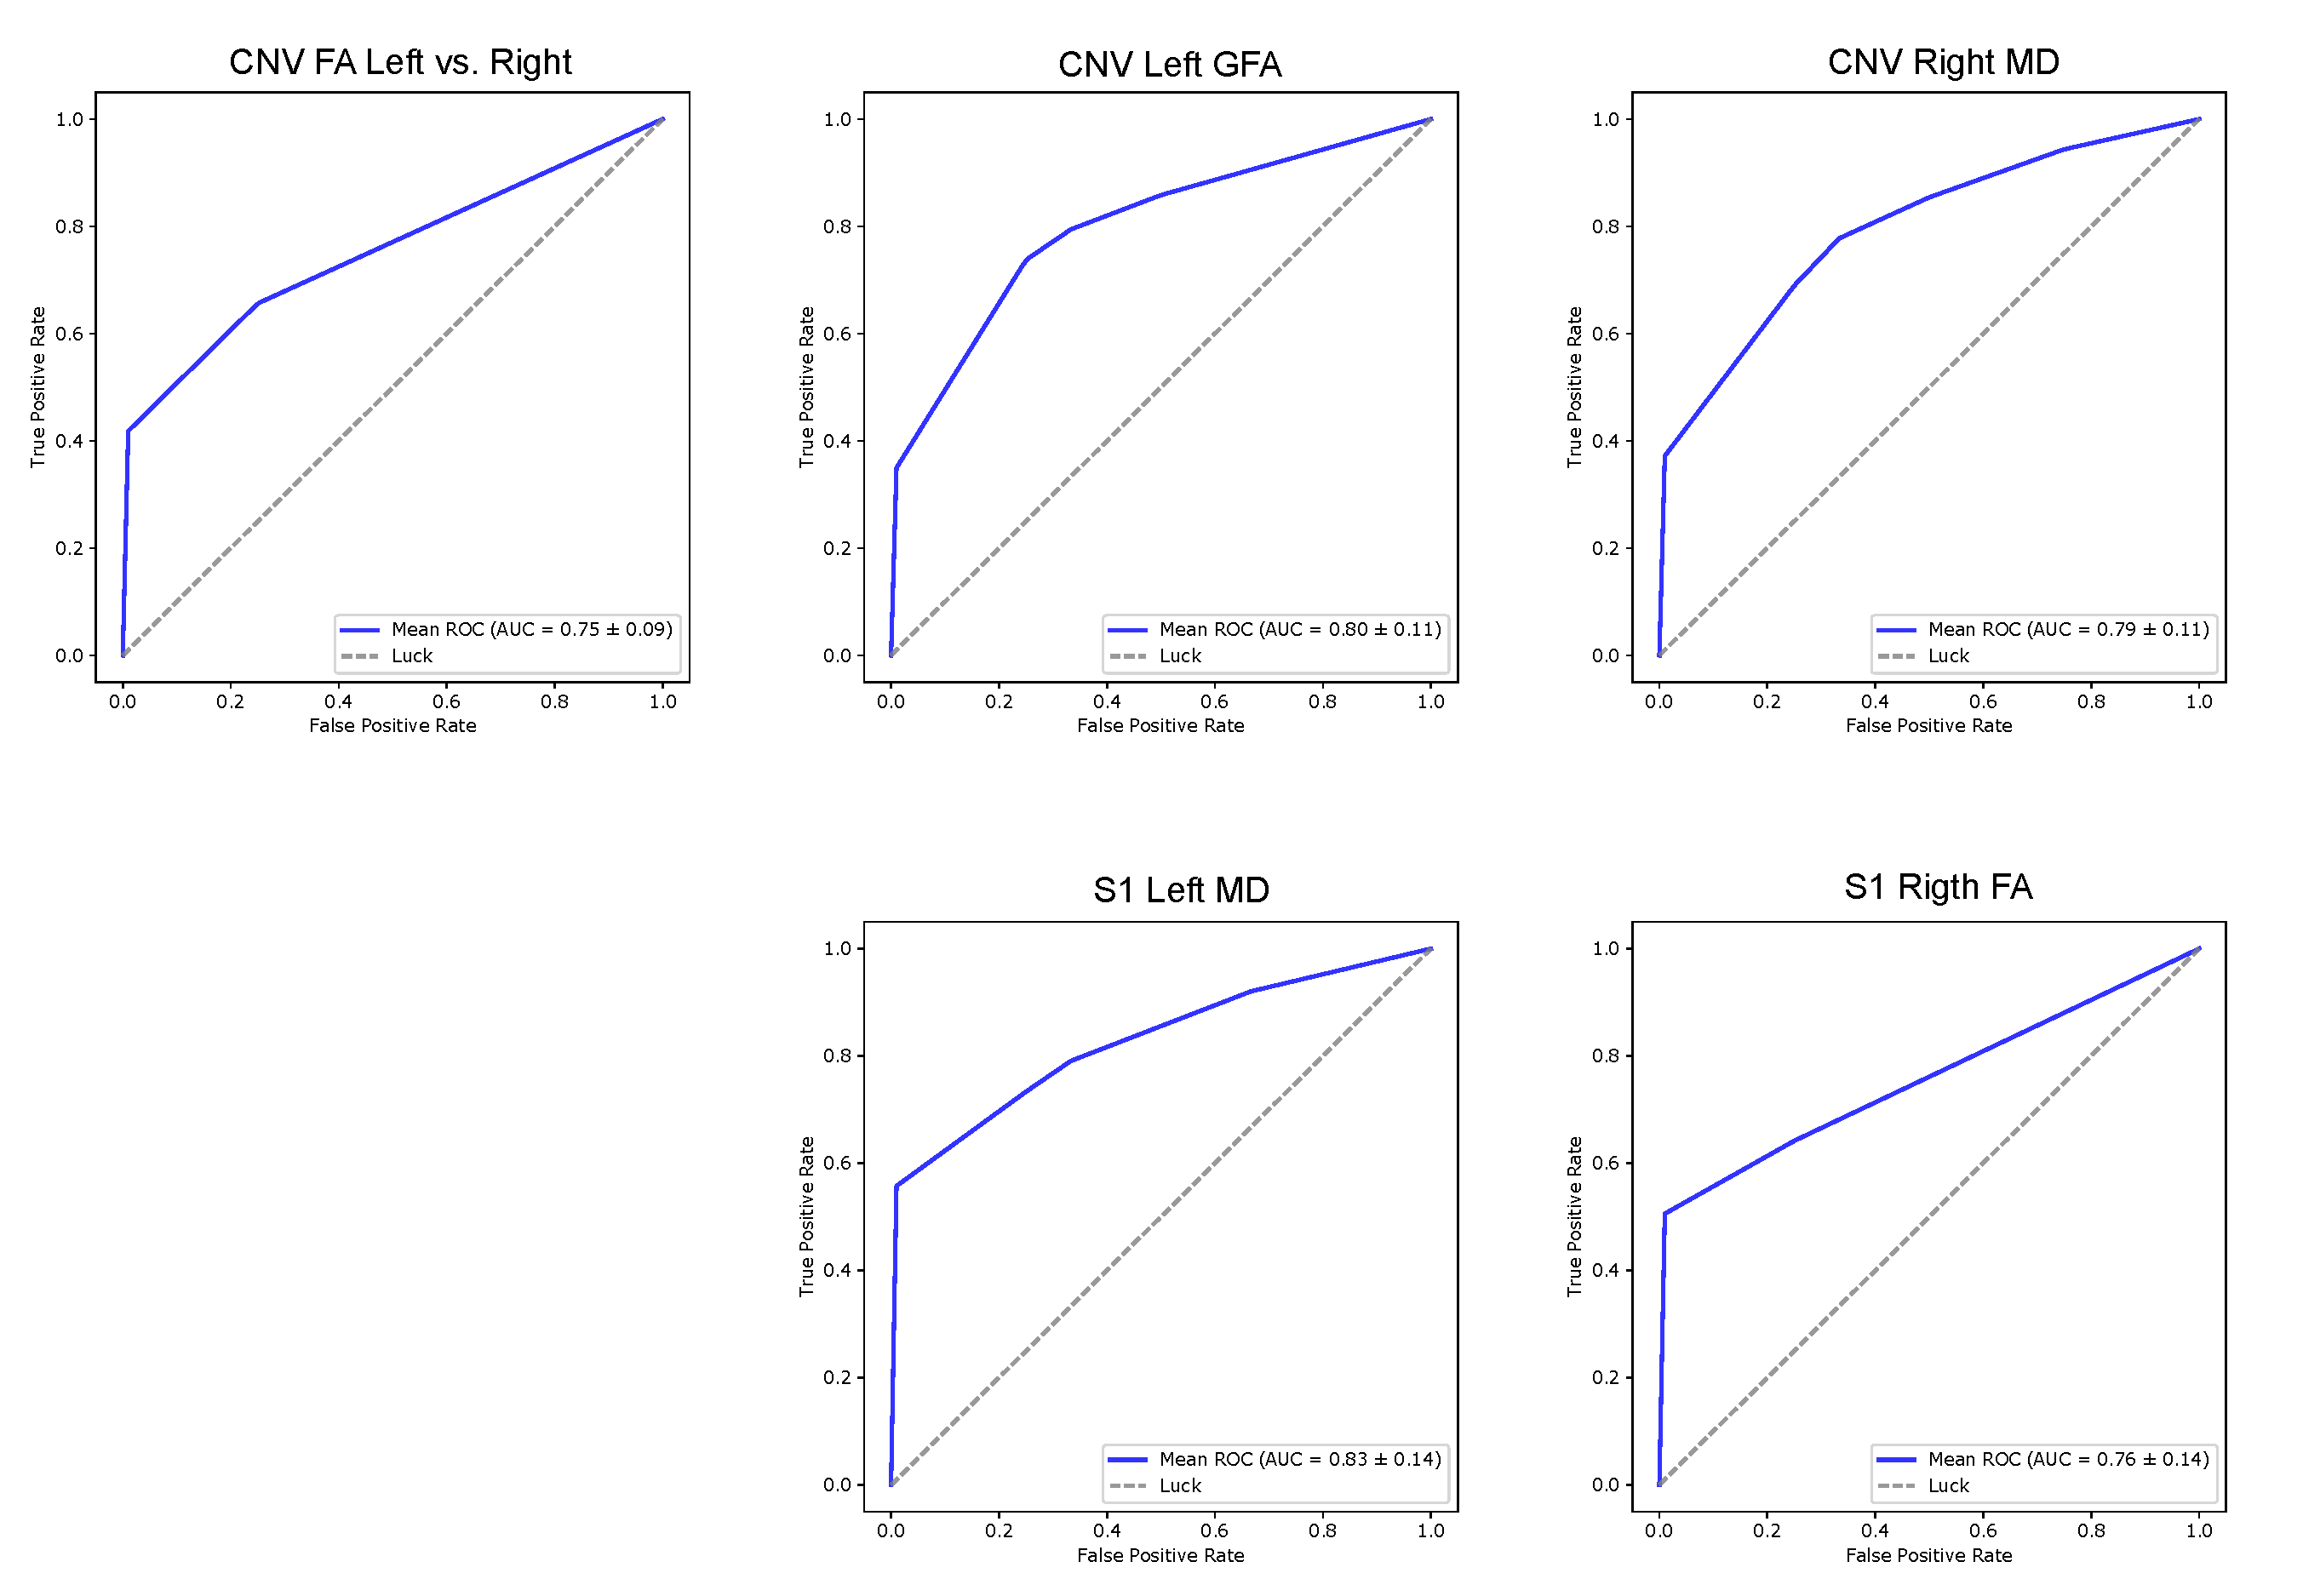
\includegraphics[width=\linewidth]{figure-roc.pdf}
\caption{ROC curves of the top performing classifiers}
\label{fig:GPfigure6}
\end{figure}

\section{Discussion}
The study is the first instance of machine learning discrimination of TN vs. Controls with specific white matter analysis, using group-wise merged along-the-track tractography. In essence, we have demonstrated a fully-automated, end-to-end tractography and machine learning platform that is capable of discriminate TN from white-matter diffusivity with greater than 80\% accuracy solely from white-matter measures. We reproduced previous findings of TN diffusivity changes along the CN V with much higher regional specificity. We also examined TPT and S1 projections of the trigeminal sensory pathway.

The diffusivity measures of CN V reproduced our previous findings \cite{Chen2016a}, which was that cistern, REZ differentiated TN from controls. The consistent regional overlaps in the cistern/REZ region of the right (affected) CN V in MD, RD, AD shows the ability for the GP classifiers to auto-converge to focal white-matter abnormality. The left versus right GP classifier placed left-right differences at the cistern segment, in agreement with the pathophysiology of TN. The regional findings on left versus controls suggest that there is bilateral differences in CN V myeline in unilateral TN, despite the lack of symptoms on the unaffected side. The left regions also situate into the brainstem segments. It is possible that the left CN V is affected by global descending pain modulation, and warrant further investigation. 

The S1 delineation was consistent, due to full automation using SAGIT and the incorporation of Freesurfer cortical segmentation maps. Reproducing streamlines into the face-region of S1 cortex in multiple subjects was difficult previously due to individual variations, as well as the multi-directional fiber crossings in the coronal radiata. Previous studies have suggested that S1 have key involvement in pain location discrimination \cite{bushnell1999pain}, and are found to have grey-matter abnormalities in TN pain \cite{Desouza2013c}. Our finding that the left (affected) thalamocortical S1 projection is uniquely different close to the cortex suggest that deep cortical white-matter/grey-matter changes may be related depending on the locality. 

The TPT delineations showed that decussation pathway tractography is possibly asymmetric. It is not clear if the asymmetry is a neuroanatomically factual, or an artifact from either algorithmic bias or partial volume bias of the underlying DWI. Resolving crossing fiber is still a difficult task in tractography, and while there are validations against MR phantoms, the anatomical validity of these methods can only be extrapolated, and the interpretation must involve anatomical priors from experts.  

We included GFA to investigate its potential for measuring deep white-matter diffusivity, as it is the most well-known non-Gaussian diffusivity metric. However S1 results demonstrated that it is not effective in pinpoint deep white-matter abnormalities. GFA performed well in CN V, but not to any substantially degree than the Gaussian-base diffusivity metrics. 

Overall the GP classifiers resulted in higher precision when compared to accuracy. The overlapping regions revealed differences in localizations that may very well have been missed with singular diffusivity metric analysis. This suggests that cross-metric features should be considered in future studies. This would drastically increase the feature complexity, and thereby require subsequent demand in the number of subjects. 

\subsubsection{Limitations}
The merged CN V delineations of all the subjects showed caudal projections towards the spinal cord. In multiple instances, diverging streamlines at the levels of the medulla strongly suggested the trigeminal spinal decussations. However the caudal projection was not available for the majority of the TN group, and it was not a consistently producible pathway. This is likely due to that 1) 3T DWI scan has a limited 2mm isovoxel resolution; It is not enough to resolve CN V, medullary and spinal cord fiber details. We have modified our scan to 1x1x3mm voxel, to gain axial plane detail for this kind of small fiber tractography from clinical scans, at the sacrifice of coronal/sagittal resolution. 2) A large percent of the TN DWI scans has severe distortions at the pontine level. Similar distortions rarely show up in Control or MS-TN scans. The reason may be due to the changes in the vertebral and basilar blood vessels that gave rise to EPI distortions in these patients. These distortions narrow the brainstem in the DWI image, and when combined with limited resolution, making tractography delineations even more difficult. Therefore, it is highly recommended to perform reverse-blip DWI acquisitions in patients with cerebral vessel irregularities as part of MR DWI clinical practice. 

The diffusivity metrics of the deeper white matter structures remains difficult to interpret, due to the complex crossing fibers in these regions. Although metrics such as FA are popular in current neuroimaging literature, they nevertheless are derived from the Gaussian tensor model, which cannot adequately describe cross-fiber regional dynamics. For example, in the crossing-fiber region of healthy tissue, where both bundles have equal myelin and axonal integrity, will have a low FA score due to a spherical tensor; its AD and RD will be roughly equal, and therefore MD will be higher. In a pathological cross region, where only one bundle is healthy, the FA increases due to the diffusivity bias in one direction; the RD will be lower, and MD will be lower as well. Moreover, in diverging and converging structures, as well as in multi-crossing regions such as the corona radiata, the interpretations of Gaussian-based diffusivity metrics become even more unclear. Therefore, it is imperative that interpretable diffusivity measures for crossing regions be established and adopted by the neuroimaging tractography field for future studies. 

\subsection{Conclusions}
We have demonstrated the first instance of group-wise merged along-the-track tractography analysis of TN vs. control. We have achieved examination of specific and targeted anatomy at a group level involving both healthy and pathological brain images. The method reproduced previous findings of TN diffusivity changes along the CN V with finer-grained regional specificity. We also examined TPT and S1 projections of the trigeminal sensory pathway. The study revealed that there are specific diffusivity changes on these deeper white matter structures, and demonstrated the power of along-the-tract analysis with machine-learning, which pinpoints the exact location of the diffusivity disruption at millimetre level. 
